\documentclass[
  man,
  longtable,
  nolmodern,
  notxfonts,
  notimes,
  colorlinks=true,linkcolor=blue,citecolor=blue,urlcolor=blue]{apa7}

\usepackage{amsmath}
\usepackage{amssymb}




\RequirePackage{longtable}
\RequirePackage{threeparttablex}

\makeatletter
\renewcommand{\paragraph}{\@startsection{paragraph}{4}{\parindent}%
	{0\baselineskip \@plus 0.2ex \@minus 0.2ex}%
	{-.5em}%
	{\normalfont\normalsize\bfseries\typesectitle}}

\renewcommand{\subparagraph}[1]{\@startsection{subparagraph}{5}{0.5em}%
	{0\baselineskip \@plus 0.2ex \@minus 0.2ex}%
	{-\z@\relax}%
	{\normalfont\normalsize\bfseries\itshape\hspace{\parindent}{#1}\textit{\addperi}}{\relax}}
\makeatother




\usepackage{longtable, booktabs, multirow, multicol, colortbl, hhline, caption, array, float, xpatch}
\usepackage{subcaption}


\renewcommand\thesubfigure{\Alph{subfigure}}
\setcounter{topnumber}{2}
\setcounter{bottomnumber}{2}
\setcounter{totalnumber}{4}
\renewcommand{\topfraction}{0.85}
\renewcommand{\bottomfraction}{0.85}
\renewcommand{\textfraction}{0.15}
\renewcommand{\floatpagefraction}{0.7}

\usepackage{tcolorbox}
\tcbuselibrary{listings,theorems, breakable, skins}
\usepackage{fontawesome5}

\definecolor{quarto-callout-color}{HTML}{909090}
\definecolor{quarto-callout-note-color}{HTML}{0758E5}
\definecolor{quarto-callout-important-color}{HTML}{CC1914}
\definecolor{quarto-callout-warning-color}{HTML}{EB9113}
\definecolor{quarto-callout-tip-color}{HTML}{00A047}
\definecolor{quarto-callout-caution-color}{HTML}{FC5300}
\definecolor{quarto-callout-color-frame}{HTML}{ACACAC}
\definecolor{quarto-callout-note-color-frame}{HTML}{4582EC}
\definecolor{quarto-callout-important-color-frame}{HTML}{D9534F}
\definecolor{quarto-callout-warning-color-frame}{HTML}{F0AD4E}
\definecolor{quarto-callout-tip-color-frame}{HTML}{02B875}
\definecolor{quarto-callout-caution-color-frame}{HTML}{FD7E14}

%\newlength\Oldarrayrulewidth
%\newlength\Oldtabcolsep


\usepackage{hyperref}



\usepackage{color}
\usepackage{fancyvrb}
\newcommand{\VerbBar}{|}
\newcommand{\VERB}{\Verb[commandchars=\\\{\}]}
\DefineVerbatimEnvironment{Highlighting}{Verbatim}{commandchars=\\\{\}}
% Add ',fontsize=\small' for more characters per line
\usepackage{framed}
\definecolor{shadecolor}{RGB}{241,243,245}
\newenvironment{Shaded}{\begin{snugshade}}{\end{snugshade}}
\newcommand{\AlertTok}[1]{\textcolor[rgb]{0.68,0.00,0.00}{#1}}
\newcommand{\AnnotationTok}[1]{\textcolor[rgb]{0.37,0.37,0.37}{#1}}
\newcommand{\AttributeTok}[1]{\textcolor[rgb]{0.40,0.45,0.13}{#1}}
\newcommand{\BaseNTok}[1]{\textcolor[rgb]{0.68,0.00,0.00}{#1}}
\newcommand{\BuiltInTok}[1]{\textcolor[rgb]{0.00,0.23,0.31}{#1}}
\newcommand{\CharTok}[1]{\textcolor[rgb]{0.13,0.47,0.30}{#1}}
\newcommand{\CommentTok}[1]{\textcolor[rgb]{0.37,0.37,0.37}{#1}}
\newcommand{\CommentVarTok}[1]{\textcolor[rgb]{0.37,0.37,0.37}{\textit{#1}}}
\newcommand{\ConstantTok}[1]{\textcolor[rgb]{0.56,0.35,0.01}{#1}}
\newcommand{\ControlFlowTok}[1]{\textcolor[rgb]{0.00,0.23,0.31}{\textbf{#1}}}
\newcommand{\DataTypeTok}[1]{\textcolor[rgb]{0.68,0.00,0.00}{#1}}
\newcommand{\DecValTok}[1]{\textcolor[rgb]{0.68,0.00,0.00}{#1}}
\newcommand{\DocumentationTok}[1]{\textcolor[rgb]{0.37,0.37,0.37}{\textit{#1}}}
\newcommand{\ErrorTok}[1]{\textcolor[rgb]{0.68,0.00,0.00}{#1}}
\newcommand{\ExtensionTok}[1]{\textcolor[rgb]{0.00,0.23,0.31}{#1}}
\newcommand{\FloatTok}[1]{\textcolor[rgb]{0.68,0.00,0.00}{#1}}
\newcommand{\FunctionTok}[1]{\textcolor[rgb]{0.28,0.35,0.67}{#1}}
\newcommand{\ImportTok}[1]{\textcolor[rgb]{0.00,0.46,0.62}{#1}}
\newcommand{\InformationTok}[1]{\textcolor[rgb]{0.37,0.37,0.37}{#1}}
\newcommand{\KeywordTok}[1]{\textcolor[rgb]{0.00,0.23,0.31}{\textbf{#1}}}
\newcommand{\NormalTok}[1]{\textcolor[rgb]{0.00,0.23,0.31}{#1}}
\newcommand{\OperatorTok}[1]{\textcolor[rgb]{0.37,0.37,0.37}{#1}}
\newcommand{\OtherTok}[1]{\textcolor[rgb]{0.00,0.23,0.31}{#1}}
\newcommand{\PreprocessorTok}[1]{\textcolor[rgb]{0.68,0.00,0.00}{#1}}
\newcommand{\RegionMarkerTok}[1]{\textcolor[rgb]{0.00,0.23,0.31}{#1}}
\newcommand{\SpecialCharTok}[1]{\textcolor[rgb]{0.37,0.37,0.37}{#1}}
\newcommand{\SpecialStringTok}[1]{\textcolor[rgb]{0.13,0.47,0.30}{#1}}
\newcommand{\StringTok}[1]{\textcolor[rgb]{0.13,0.47,0.30}{#1}}
\newcommand{\VariableTok}[1]{\textcolor[rgb]{0.07,0.07,0.07}{#1}}
\newcommand{\VerbatimStringTok}[1]{\textcolor[rgb]{0.13,0.47,0.30}{#1}}
\newcommand{\WarningTok}[1]{\textcolor[rgb]{0.37,0.37,0.37}{\textit{#1}}}

\providecommand{\tightlist}{%
  \setlength{\itemsep}{0pt}\setlength{\parskip}{0pt}}
\usepackage{longtable,booktabs,array}
\usepackage{calc} % for calculating minipage widths
% Correct order of tables after \paragraph or \subparagraph
\usepackage{etoolbox}
\makeatletter
\patchcmd\longtable{\par}{\if@noskipsec\mbox{}\fi\par}{}{}
\makeatother
% Allow footnotes in longtable head/foot
\IfFileExists{footnotehyper.sty}{\usepackage{footnotehyper}}{\usepackage{footnote}}
\makesavenoteenv{longtable}

\usepackage{graphicx}
\makeatletter
\def\maxwidth{\ifdim\Gin@nat@width>\linewidth\linewidth\else\Gin@nat@width\fi}
\def\maxheight{\ifdim\Gin@nat@height>\textheight\textheight\else\Gin@nat@height\fi}
\makeatother
% Scale images if necessary, so that they will not overflow the page
% margins by default, and it is still possible to overwrite the defaults
% using explicit options in \includegraphics[width, height, ...]{}
\setkeys{Gin}{width=\maxwidth,height=\maxheight,keepaspectratio}
% Set default figure placement to htbp
\makeatletter
\def\fps@figure{htbp}
\makeatother


% definitions for citeproc citations
\NewDocumentCommand\citeproctext{}{}
\NewDocumentCommand\citeproc{mm}{%
  \begingroup\def\citeproctext{#2}\cite{#1}\endgroup}
\makeatletter
 % allow citations to break across lines
 \let\@cite@ofmt\@firstofone
 % avoid brackets around text for \cite:
 \def\@biblabel#1{}
 \def\@cite#1#2{{#1\if@tempswa , #2\fi}}
\makeatother
\newlength{\cslhangindent}
\setlength{\cslhangindent}{1.5em}
\newlength{\csllabelwidth}
\setlength{\csllabelwidth}{3em}
\newenvironment{CSLReferences}[2] % #1 hanging-indent, #2 entry-spacing
 {\begin{list}{}{%
  \setlength{\itemindent}{0pt}
  \setlength{\leftmargin}{0pt}
  \setlength{\parsep}{0pt}
  % turn on hanging indent if param 1 is 1
  \ifodd #1
   \setlength{\leftmargin}{\cslhangindent}
   \setlength{\itemindent}{-1\cslhangindent}
  \fi
  % set entry spacing
  \setlength{\itemsep}{#2\baselineskip}}}
 {\end{list}}
\usepackage{calc}
\newcommand{\CSLBlock}[1]{\hfill\break\parbox[t]{\linewidth}{\strut\ignorespaces#1\strut}}
\newcommand{\CSLLeftMargin}[1]{\parbox[t]{\csllabelwidth}{\strut#1\strut}}
\newcommand{\CSLRightInline}[1]{\parbox[t]{\linewidth - \csllabelwidth}{\strut#1\strut}}
\newcommand{\CSLIndent}[1]{\hspace{\cslhangindent}#1}





\usepackage{newtx}

\defaultfontfeatures{Scale=MatchLowercase}
\defaultfontfeatures[\rmfamily]{Ligatures=TeX,Scale=1}





\title{Why Risk it, When You Can \{rix\} it: A Tutorial for
Computational Reproducibility Focused on Simulation Studies}


\shorttitle{Reproducibility with rix}


\usepackage{etoolbox}









\authorsnames[{1},{2},{3}]{Felipe Fontana Vieira,Jason Geller,Bruno
Rodrigues}







\authorsaffiliations{
{Department of Data Analysis, Ghent University},{Department of
Psychology and Neuroscience, Boston College},{Statistics and Data
Strategy Departments, Ministry of Research and Higher Education,
Luxembourg}}




\leftheader{Vieira, Geller and Rodrigues}



\abstract{Reproducibility remains limited in psychology, in part because
reproducibility exists on a spectrum -- from sharing isolated code
fragments to providing fully executable pipelines that ensure identical
results. This article introduces Nix and the \{rix\} R package as a way
to provide a comprehensive solution for achieving full computational
reproducibility in simulation studies. Building on this, we also
demonstrate a tutorial on how to use \{rix\} to obtain a reproducible
manuscript using the apaquarto extension. }

\keywords{reproducibility, Nix, simulation studies, R, computational
methods}

\authornote{ 

\par{       }
\par{Correspondence concerning this article should be addressed
to Felipe Fontana
Vieira, Email: \href{mailto:felipe.fontanavieira@ugent.be}{felipe.fontanavieira@ugent.be}}
}

\makeatletter
\let\endoldlt\endlongtable
\def\endlongtable{
\hline
\endoldlt
}
\makeatother
\RequirePackage{longtable}
\DeclareDelayedFloatFlavor{longtable}{table}

\urlstyle{same}



\usepackage{setspace}
\usepackage{etoolbox}
\raggedbottom
% Single-space code blocks
\AtBeginEnvironment{Shaded}{\singlespacing}
\AtBeginEnvironment{verbatim}{\singlespacing}
\makeatletter
\@ifpackageloaded{caption}{}{\usepackage{caption}}
\AtBeginDocument{%
\ifdefined\contentsname
  \renewcommand*\contentsname{Table of contents}
\else
  \newcommand\contentsname{Table of contents}
\fi
\ifdefined\listfigurename
  \renewcommand*\listfigurename{List of Figures}
\else
  \newcommand\listfigurename{List of Figures}
\fi
\ifdefined\listtablename
  \renewcommand*\listtablename{List of Tables}
\else
  \newcommand\listtablename{List of Tables}
\fi
\ifdefined\figurename
  \renewcommand*\figurename{Figure}
\else
  \newcommand\figurename{Figure}
\fi
\ifdefined\tablename
  \renewcommand*\tablename{Table}
\else
  \newcommand\tablename{Table}
\fi
}
\@ifpackageloaded{float}{}{\usepackage{float}}
\floatstyle{ruled}
\@ifundefined{c@chapter}{\newfloat{codelisting}{h}{lop}}{\newfloat{codelisting}{h}{lop}[chapter]}
\floatname{codelisting}{Listing}
\newcommand*\listoflistings{\listof{codelisting}{List of Listings}}
\makeatother
\makeatletter
\makeatother
\makeatletter
\@ifpackageloaded{caption}{}{\usepackage{caption}}
\@ifpackageloaded{subcaption}{}{\usepackage{subcaption}}
\makeatother

% From https://tex.stackexchange.com/a/645996/211326
%%% apa7 doesn't want to add appendix section titles in the toc
%%% let's make it do it
\makeatletter
\xpatchcmd{\appendix}
  {\par}
  {\addcontentsline{toc}{section}{\@currentlabelname}\par}
  {}{}
\makeatother

%% Disable longtable counter
%% https://tex.stackexchange.com/a/248395/211326

\usepackage{etoolbox}

\makeatletter
\patchcmd{\LT@caption}
  {\bgroup}
  {\bgroup\global\LTpatch@captiontrue}
  {}{}
\patchcmd{\longtable}
  {\par}
  {\par\global\LTpatch@captionfalse}
  {}{}
\apptocmd{\endlongtable}
  {\ifLTpatch@caption\else\addtocounter{table}{-1}\fi}
  {}{}
\newif\ifLTpatch@caption
\makeatother

\begin{document}

\maketitle




\setlength\LTleft{0pt}




Psychological science is in the midst of a credibility revolution, which
has prompted substantial progress in how research is conducted and
evaluated (\citeproc{ref-vazire2018}{Vazire, 2018}). Yet, despite
notable progress, a key cornerstone of science, reproducibility (i.e.,
the ability to precisely reproduce the results of a study or studies
based on provided data, code, materials, and software/hardware) remains
limited (\citeproc{ref-hardwicke2020}{Hardwicke et al., 2020}). Hence,
ensuring reproducibility remains an open and pressing challenge for
psychological science.

Addressing this gap is complicated by the fact that reproducibility is
not a binary feature but instead exists along a continuum
(\citeproc{ref-peng_2011}{Peng, 2011}). At the lower end,
reproducibility may be interpreted as sharing only a manuscript. Further
along the spectrum, it may involve providing partial code, complete
analysis scripts, or publicly accessible datasets. At the highest level,
reproducibility entails documenting a fully specified computational
environment that allows others to recreate identical results---from raw
data to final manuscript output---with minimal friction. As a result,
researchers may implicitly target different points on this continuum and
efforts to improve reproducibility can diverge substantially in both
goals and implementation.

Open science initiatives have made considerable progress in encouraging
movement along this continuum. For example, journals have begun offering
open-science badges (\citeproc{ref-kidwell_etall_2016}{Kidwell et al.,
2016}) and platforms like the Open Science Framework (OSF) have created
``challenges'' to make data and code sharing increasingly routine
(\citeproc{ref-levenstein_lyle_2018}{Levenstein \& Lyle, 2018}).
However, these efforts largely occupy the lower and middle portions of
the continuum, emphasizing what is shared rather than how shared
materials can be executed in practice.

Data and code are never fully self-sufficient to reproduce a set of
findings. Assuming the data and code are error-free, reproducibility
depends on a hierarchy of software components---collectively referred to
as \emph{dependencies}---including the programming language version, the
packages used in the analysis, and the system libraries on which those
packages rely. When these dependencies differ from those used in the
original analysis, code may fail, behave inconsistently across machines,
or yield conflicting numerical results
(\citeproc{ref-baker_etall_2024}{Baker et al., 2024};
\citeproc{ref-glatard_etall_2015}{Glatard et al., 2015};
\citeproc{ref-hodges_etall_2023}{Hodges et al., 2023};
\citeproc{ref-nosek_etall_2022}{Nosek et al., 2022}). These issues are
particularly acute for simulation studies, which rely on complex
codebases, versioned dependencies, and intricate software configurations
(\citeproc{ref-luijken_etall_2024}{Luijken et al., 2024};
\citeproc{ref-siepe_etall_2024}{Siepe et al., 2024}).

To make this concrete, we use \emph{computational environment} to refer
to the complete software context required for an analysis to run
successfully---the programming language version, package versions,
system libraries, and operating system
(\citeproc{ref-rodrigues_2023}{Rodrigues, 2023};
\citeproc{ref-rodrigues_baumann_2026_polyglot}{Rodrigues \& Baumann,
2026}). We define \emph{computational environment reproducibility} as
the ability to reconstruct this entire set of software dependencies on
any machine and at any future time, such that executing the same code
yields the same numerical results. Empirical assessments show that
current practice falls short of this ideal. Siepe et al.
(\citeproc{ref-siepe_etall_2024}{2024}) report that nearly two-thirds of
simulation studies in psychology provide no accompanying code, and among
those that do, documentation of the computational environment is rarely
included. This gap is consequential: simulation studies inform
methodological recommendations, meaning that insufficient
reproducibility undermines confidence in those recommendations
(\citeproc{ref-luijken_etall_2024}{Luijken et al., 2024};
\citeproc{ref-white_etall_2024}{White et al., 2024}).

Arguably, these challenges persist because researchers must navigate a
fragmented landscape of solutions, each addressing only part of the
problem. Package-level managers such as \{renv\}
(\citeproc{ref-ushey_2024}{Ushey, 2024}) and \{groundhog\}
(\citeproc{ref-simonsohn_2020}{Simonsohn, 2020}) stabilize R package
versions but do not manage the R interpreter itself or the system-level
libraries those packages depend on. Workflow orchestration tools such as
\{targets\} (\citeproc{ref-landau_2021}{Landau, 2021}) and Make
(\citeproc{ref-feldman_1979}{Feldman, 1979}) support reproducibility in
a different sense: they specify the structure of an analysis by
formalizing the order in which steps should run and by tracking
dependencies among intermediate results. These tools clarify \emph{how}
an analysis proceeds, but they assume that the software stack required
to run each step is already stable. Containerization tools such as
Docker, including R-focused implementations like
Rocker(\citeproc{ref-boettiger_2015}{Boettiger, 2015};
\citeproc{ref-boettiger_eddelbuettel_2017}{Boettiger \& Eddelbuettel,
2017}) offer a more comprehensive approach by bundling the full
environment---operating system, system libraries, interpreter versions,
and packages---into a single executable image. Yet their use requires
familiarity with Linux system administration, and even containerization
may suffer from temporal drift when Dockerfiles rely on mutable upstream
repositories (\citeproc{ref-malka2024}{Malka et al., 2024}). For a
detailed comparison of these tools and their limitations, see Rodrigues
and Baumann (\citeproc{ref-rodrigues_baumann_2026_polyglot}{2026}).
Researchers thus face a difficult choice between solutions that are
accessible but incomplete or approaches that are powerful but demand
technical expertise.

In this article, therefore, we focus specifically on computational
environment reproducibility as the foundation upon which other
reproducibility practices depend. For that, we introduce Nix
(\citeproc{ref-dolstra_etall_2004}{Dolstra et al., 2004}), a functional
software ecosystem designed to make software installation deterministic,
and \{rix\} (\citeproc{ref-rodrigues_baumann_2025}{Rodrigues \& Baumann,
2025}), an R interface that allows researchers to use Nix without
needing deep knowledge of its underlying language or infrastructure. Our
objective is not to introduce a specific workflow orchestration system
or to prescribe a particular analytic structure. Instead, we aim to show
how Nix and \{rix\} can establish a stable, cross-platform environment
within which any analysis---whether organized in simple, documented
script sequences (e.g., .R files that \texttt{source()} others), through
more formal orchestration tools (e.g., targets) or embedded as code
chunks in \texttt{.Rmd} or \texttt{.qmd} ---can be executed reliably.

We illustrate these ideas through a reproducible simulation study
conducted in R, culminating in an automated APA-formatted manuscript
generated with \texttt{apaquarto}
(\citeproc{ref-schneider_2024}{Schneider, 2024}). Although the example
centers on R because of its prominence in psychological methodology, the
principles underlying environment reproducibility apply equally to other
languages, including Python and Julia, and to different development
environments such as RStudio, VS Code, Emacs, or Positron. Later in the
article, we briefly comment on rixpress
(\citeproc{ref-rixpress}{Rodrigues, 2025}), which extends Nix-based
reproducibility to workflows spanning multiple languages. Throughout,
our emphasis remains squarely on the reproducibility of computational
environments as the essential basis for transparent, reliable, and
durable scientific workflows.

\section{A Practical Example: Setting up a Reproducible Simulation Study
with
\{rix\}}\label{a-practical-example-setting-up-a-reproducible-simulation-study-with-rix}

Imagine you have just been awarded a grant to conduct a large-scale
simulation study. The study is designed to evaluate the performance of a
statistical estimator under varying data-generating conditions (see
Appendix A for full technical details). This tutorial is organized
around this scenario. We use this stylized example to ground our
discussion into a typical methods section, but readers can follow the
tutorial without engaging deeply with the simulation itself.

In practice, simulation studies are typically implemented across
multiple component files, each corresponding to a distinct analytical
stage. In our case, the simulation is organized into five sequential
scripts: data generation (\texttt{01\_data\_generation.R}), model
specification (\texttt{02\_models.R}), simulation execution
(\texttt{03\_run\_simulation.R}), performance metric calculation
(\texttt{04\_performance\_metrics.R}), and results visualization
(\texttt{05\_plots.R}). This modular structure reflects common practice
and facilitates development and debugging. However, because our focus is
on the reproducibility of the \emph{entire manuscript}, we embed all
code directly within this document as executable chunks in a single .qmd
file. When rendered, the simulation runs from start to finish, producing
results and figures automatically. This approach would be impractical
for many real-world simulation studies, which are often too
computationally intensive. We return to this trade-off later in the
tutorial.

Now suppose a researcher attempts to reproduce the simulation results
reported in the article. What might prevent them from obtaining
identical outcomes? The natural first concern is package versioning.
Installing R packages at a later time may lead to errors if functions
have been renamed or deprecated (e.g.,
\texttt{lavaan:::lav\_utils\_get\_ancestors} renamed to
\texttt{lavaan:::lav\_graph\_get\_ancestors()}), or to subtly different
results due to changes in default settings or numerical implementations
(e.g., \texttt{stringsAsFactors} defaulting to FALSE as of R 4.0).
Beyond R packages themselves, many packages rely on system-level
libraries that must be installed separately from R. Our simulation
illustrates this dependency structure directly: the \{rvinecopulib\}
package interfaces with a C++ backend and links against external
libraries such as Boost, Eigen, and RcppThread
(\citeproc{ref-rvinecopulib}{Nagler \& Vatter, 2025}).

The R language version introduces another layer of dependency. Code
written for R 4.0 may rely on syntax or functionality that is
unavailable in earlier versions (e.g., the native pipe
\texttt{\textbar{}\textgreater{}} introduced in R 4.1). More subtly,
changes to R's random number generation across major versions mean that
identical code executed with the same seed can nevertheless produce
different random sequences (\citeproc{ref-ottoboni_stark_2018}{Ottoboni
\& Stark, 2018}). For simulation studies---where specific random draws
often underpin reported results---this version sensitivity is
consequential.

Finally, when analyses are embedded in a literate programming workflow
(i.e., documents that combine narrative text and executable code)
additional layers of software dependencies arise. For example, rendering
R Markdown (\texttt{.rmd}) or Quarto documents (\texttt{.qmd}) requires
both a document conversion tool (e.g., Pandoc, which converts
\texttt{.rmd} or \texttt{.qmd} files into formats such as PDF or HTML)
and a typesetting system such as a LaTeX distribution or Typst. Each of
these components introduces its own versioning constraints and
platform-specific installation requirements. Taken together, these
layers highlight that reproducibility depends not only on code and data,
but also on the broader computational environment in which analyses are
executed.

\section{Nix and \{rix\}: A Comprehensive
Solution}\label{nix-and-rix-a-comprehensive-solution}

A potential solution to the above issue is Nix
(\citeproc{ref-dolstra_etall_2004}{Dolstra et al., 2004}). Nix is a
software ecosystem centered on a purely functional package manager and
build system designed to make software environments reproducible,
declarative, and isolated across platforms (think Apple's or Android's
application store). In practical terms, this means that Nix allows
researchers to specify \emph{exactly} which versions of programming
languages, packages, and system libraries an analysis requires, and to
recreate that same environment reliably on another machine.

Unlike familiar tools such as \texttt{install.packages()} in R,
\texttt{apt-get} on Linux, or \texttt{uv} in Python---which typically
manage only a single layer of the software stack---Nix handles language
versions, package versions, and system-level dependencies within a
single framework (\citeproc{ref-rodrigues_baumann_2025}{Rodrigues \&
Baumann, 2025}). Rather than installing software into shared system
directories, Nix builds each environment as an explicit, self-contained
specification. As a result, multiple environments can coexist without
conflict, and analyses can be rerun months or years later under
identical computational conditions.

This unified approach directly addresses the fragmented landscape
described above. Where researchers would otherwise need to coordinate
separate tools for package management, interpreter versions, and system
dependencies, Nix brings all three together within a single declarative
model, lowering the barrier to fully reproducible computational
workflows.

\subsection{Core Principles}\label{core-principles}

Rather than installing software into global directories (e.g.,
\texttt{/usr/lib}), Nix places every package in its own directory under
\texttt{/nix/store}. Each package path contains a cryptographic hash
representing its precise inputs---source code, dependencies, and build
instructions. Because these paths are content-addressed, multiple
versions of the same software can coexist without conflict. A researcher
can, for example, maintain projects requiring R 4.1.0 and R 4.3.3 side
by side, or use different package versions across analyses, switching
between them seamlessly (\citeproc{ref-rodrigues_baumann_2025}{Rodrigues
\& Baumann, 2025}).

The Nix ecosystem is built around nixpkgs, a version-controlled
repository comprising more than 120,000 packages, including nearly all
of CRAN and Bioconductor. By pinning a specific commit or date,
researchers freeze the entire software stack---R itself, R packages, and
all system libraries---at that point in time. This eliminates the
system-dependency problems that tools like \{renv\} cannot address
(\citeproc{ref-rodrigues_baumann_2025}{Rodrigues \& Baumann, 2025}).
This architecture also ensures stability over time. Empirical work has
shown strong rebuildability and reproducibility rates for historical
nixpkgs snapshots
(\citeproc{ref-rodrigues_baumann_2026_polyglot}{Rodrigues \& Baumann,
2026}). Combined with binary caches, which often allow environments to
materialize in seconds, Nix becomes practical for interactive research
workflows (\citeproc{ref-rodrigues_baumann_2025}{Rodrigues \& Baumann,
2025}).

\subsection{The \{rix\} Package: R Interface to
Nix}\label{the-rix-package-r-interface-to-nix}

Nix expressions are written in a dedicated functional language
unfamiliar to most researchers. The \{rix\} package removes this barrier
by providing an R-native interface. A single call to \texttt{rix()}
generates complete Nix configurations from standard R syntax, specifying
R versions, CRAN packages, system libraries, and even Python or Julia
components when required. Users never need to read or write Nix code
directly, as \{rix\} performs the translation automatically
(\citeproc{ref-rodrigues_baumann_2025}{Rodrigues \& Baumann, 2025}).

A key feature of \{rix\} is its integration with rstats-on-nix, a
community-maintained fork offering daily CRAN snapshots and weekly
tested environments on Linux and macOS. Researchers can request, for
example, \texttt{rix(date\ =\ "2024-12-14")} to obtain a validated and
reproducible environment without manually assessing compatibility. After
the configuration is generated, \texttt{nix\_build()} instantiates the
environment, and binary caches typically allow this to complete within
seconds (\citeproc{ref-rodrigues_baumann_2025}{Rodrigues \& Baumann,
2025}).

Although Nix is capable of replacing tools like Docker for isolation or
\{renv\} for package management, it does not require an all-or-nothing
transition. Researchers can adopt it gradually and use it alongside
familiar tooling. For instance, by building Docker images with Nix,
converting existing \{renv\} lockfiles, or running \{targets\} pipelines
within a Nix-defined environment
(\citeproc{ref-rodrigues_baumann_2025}{Rodrigues \& Baumann, 2025}).
This allows Nix to strengthen reproducibility while preserving
established workflows. For projects requiring more sophisticated
pipeline management, \{rixpress\} extends Nix's guarantees to workflow
orchestration, enabling step-level isolation across languages, though
such capabilities lie beyond the present focus on environment
reproducibility. We will come back to this after the tutorial.

\subsection{Step I: Installing Nix and
\{rix\}}\label{step-i-installing-nix-and-rix}

Before proceeding, both Nix and the \{rix\} R package need to be
installed. Installation procedures differ across operating systems
(Windows via WSL2, Linux, and macOS), and detailed, up-to-date
instructions are maintained in the official \{rix\} documentation:

\begin{itemize}
\tightlist
\item
  \textbf{Linux and Windows (WSL2)}:
  \url{https://docs.ropensci.org/rix/articles/b1-setting-up-and-using-rix-on-linux-and-windows.html}
\item
  \textbf{macOS}:
  \url{https://docs.ropensci.org/rix/articles/b2-setting-up-and-using-rix-on-macos.html}
\end{itemize}

Once Nix is installed\footnote{It is worth noting that \{rix\} can
  generate Nix expressions even without Nix installed on your
  system---you can write a \texttt{default.nix} file without Nix, but
  you cannot build or enter the resulting environment unless Nix is
  installed (\citeproc{ref-rodrigues_baumann_2025}{Rodrigues \& Baumann,
  2025}).}, there are two ways to access \{rix\}, depending on whether R
is already installed on your system.

If R is already installed, \{rix\} can be installed from CRAN or from
GitHub for the development version (Listing~\ref{lst-install-rix-cran}):

\begin{codelisting}

\caption{\label{lst-install-rix-cran}Installing \{rix\} from CRAN or
developmental version}

\centering{

\begin{Shaded}
\begin{Highlighting}[]
\CommentTok{\# CRAN}
\FunctionTok{install.packages}\NormalTok{(}\StringTok{"rix"}\NormalTok{) }
\CommentTok{\# Developmental}
\FunctionTok{install.packages}\NormalTok{(}
  \StringTok{"rix"}\NormalTok{,}
  \AttributeTok{repos =} \FunctionTok{c}\NormalTok{(}
    \StringTok{"https://ropensci.r{-}universe.dev"}
\NormalTok{  )}
\NormalTok{)}
\end{Highlighting}
\end{Shaded}

}

\end{codelisting}%

If R is not installed, Nix can be used to drop directly into an R
session with \{rix\} available. Running the command in
Listing~\ref{lst-install-rix-nix-released} provides the CRAN version;
the command in Listing~\ref{lst-install-rix-nix-dev} provides the
development version:

\begin{codelisting}

\caption{\label{lst-install-rix-nix-released}R session with the released
version of \{rix\} \normalsize}

\centering{

\small

\begin{Shaded}
\begin{Highlighting}[]
\ExtensionTok{felipelfv@Felipes{-}MacBook{-}Pro}\NormalTok{ Why{-}risk{-}it{-}when{-}you{-}can{-}rix{-}it \% nix{-}shell }
  \ExtensionTok{{-}p}\NormalTok{ R rPackages.rix}
\end{Highlighting}
\end{Shaded}

}

\end{codelisting}%

\begin{codelisting}

\caption{\label{lst-install-rix-nix-dev}R session with the development
version of \{rix\} \normalsize}

\centering{

\small

\begin{Shaded}
\begin{Highlighting}[]
\ExtensionTok{felipelfv@Felipes{-}MacBook{-}Pro}\NormalTok{ Why{-}risk{-}it{-}when{-}you{-}can{-}rix{-}it \% nix{-}shell }
  \ExtensionTok{{-}{-}expr} \StringTok{"}\VariableTok{$(}\ExtensionTok{curl} \AttributeTok{{-}sl}\NormalTok{ https://raw.githubusercontent.com/ropensci/rix/}
      \ExtensionTok{main/inst/extdata/default.nix}\VariableTok{)}\StringTok{"}
\end{Highlighting}
\end{Shaded}

}

\end{codelisting}%

For the remainder of this tutorial, we assume R is already installed on
the system. Readers who accessed \{rix\} via the temporary Nix shell
should execute the subsequent R commands from within that shell until
the project-specific environment is built.

\subsection{Step II: Specifying the Computational
Environment}\label{sec-specifying-environment}

After that, we need to establish a reproducible environment by creating
a script that will generate the environment specification. We recommend
creating a file named \texttt{generate-env.R} (or similar) in the
project directory. This script will use the \texttt{rix()} function from
the \{rix\} package to produce a \texttt{default.nix} file---a
declarative specification that precisely defines all software
dependencies required for the project.

In our case, where we use literate programming for generating the
manuscript, we implement the following environment specification, which
can be found on the GitHub repository as a file named \texttt{gen-env.R}
(Listing~\ref{lst-rix-env-manuscript}):

\small

\begin{codelisting}

\caption{\label{lst-rix-env-manuscript}Environment specification for the
manuscript using rix()}

\centering{

\begin{Shaded}
\begin{Highlighting}[]
\FunctionTok{library}\NormalTok{(rix)}

\FunctionTok{rix}\NormalTok{(}
  \AttributeTok{date =} \StringTok{"2026{-}01{-}14"}\NormalTok{,}
  \AttributeTok{r\_pkgs =} \FunctionTok{c}\NormalTok{(}
    \StringTok{"rix"}\NormalTok{, }\StringTok{"quarto"}\NormalTok{, }\StringTok{"knitr"}\NormalTok{, }\StringTok{"marginaleffects"}\NormalTok{,}
    \StringTok{"simhelpers"}\NormalTok{, }\StringTok{"ggplot2"}\NormalTok{, }\StringTok{"doParallel"}\NormalTok{, }\StringTok{"doRNG"}\NormalTok{, }\StringTok{"cowplot"}\NormalTok{,}
    \StringTok{"dplyr"}\NormalTok{, }\StringTok{"svglite"}\NormalTok{, }\StringTok{"rvinecopulib"}
\NormalTok{  ),}
  \AttributeTok{system\_pkgs =} \FunctionTok{c}\NormalTok{(}\StringTok{"quarto"}\NormalTok{),}
  \AttributeTok{tex\_pkgs =} \FunctionTok{c}\NormalTok{(}\StringTok{"amsmath"}\NormalTok{, }\StringTok{"ninecolors"}\NormalTok{, }\StringTok{"apa7"}\NormalTok{, }\StringTok{"scalerel"}\NormalTok{,}
    \StringTok{"threeparttable"}\NormalTok{, }\StringTok{"threeparttablex"}\NormalTok{, }\StringTok{"endfloat"}\NormalTok{, }\StringTok{"environ"}\NormalTok{,}
    \StringTok{"multirow"}\NormalTok{, }\StringTok{"tcolorbox"}\NormalTok{, }\StringTok{"pdfcol"}\NormalTok{, }\StringTok{"tikzfill"}\NormalTok{, }\StringTok{"fontawesome5"}\NormalTok{,}
    \StringTok{"framed"}\NormalTok{, }\StringTok{"newtx"}\NormalTok{, }\StringTok{"fontaxes"}\NormalTok{, }\StringTok{"xstring"}\NormalTok{, }\StringTok{"wrapfig"}\NormalTok{, }\StringTok{"tabularray"}\NormalTok{,}
    \StringTok{"siunitx"}\NormalTok{, }\StringTok{"fvextra"}\NormalTok{, }\StringTok{"geometry"}\NormalTok{, }\StringTok{"setspace"}\NormalTok{, }\StringTok{"fancyvrb"}\NormalTok{, }
    \StringTok{"anyfontsize"}
\NormalTok{  ),}
  \AttributeTok{ide =} \StringTok{"rstudio"}\NormalTok{,}
  \AttributeTok{project\_path =} \StringTok{"."}\NormalTok{,}
  \AttributeTok{overwrite =} \ConstantTok{TRUE}
\NormalTok{)}
\end{Highlighting}
\end{Shaded}

}

\end{codelisting}%

\normalsize

Thus, note that we have more than just the R packages specified for the
simulation scripts. This happens because we also included what is needed
for the manuscript generation, not solely for the simulation code. In
Appendix B, we mention more specifically the reasons for adding each
package in \texttt{r\_pkgs()} and \texttt{tex\_pkgs()}. For now, we
focus more on clarifying the different arguments for the \texttt{rix()}
function.

\subsubsection{The Environment Generation
Script}\label{the-environment-generation-script}

The \texttt{rix()} function\footnote{For an overarching information on
  the function \texttt{rix()}, we suggest the following \{rix\}
  documentation:
  \url{https://docs.ropensci.org/rix/articles/c-using-rix-to-build-project-specific-environments.html}}
constructs this specification through a series of parameters that
collectively describe the computational environment. Each parameter
serves a distinct purpose in defining the environment's characteristics.

\paragraph{Specifying the R version.}\label{specifying-the-r-version}

Researchers must first determine which version of R to use. This can be
accomplished in two ways: The \texttt{r\_ver} argument accepts an exact
version string (e.g., ``4.3.3'') or special designations such as
``latest-upstream'' for the most recent stable release. Alternatively,
the \texttt{date} argument specifies a particular date (e.g.,
``2024-11-15''), which ensures that R and all packages correspond to the
versions available on that date. The date-based approach is generally
preferable for reproducibility, as it captures a complete snapshot of
the R ecosystem at a single point in time. For this tutorial, as shown
on top, we use the \texttt{date} parameter to ensure temporal
consistency across all software components
(\citeproc{ref-rodrigues_baumann_2025}{Rodrigues \& Baumann, 2025}) (see
\{rix\} documentation for more:
\url{https://docs.ropensci.org/rix/articles/d2-installing-system-tools-and-texlive-packages-in-a-nix-environment.html}).

\paragraph{Declaring R package
dependencies.}\label{declaring-r-package-dependencies}

The \texttt{r\_pkgs} argument accepts a character vector listing all
required R packages by their CRAN names. These packages will be
installed from the version repository corresponding to the specified
date or R version. It is important to list all packages that the
analysis will load directly; dependencies of these packages are
automatically resolved by Nix. For packages requiring specific versions
not corresponding to the chosen date, researchers can specify exact
versions using the syntax \texttt{"packagename@version"} (e.g.,
\texttt{"ggplot2@2.2.1"}). For packages available only on GitHub or
other Git repositories, the \texttt{git\_pkgs} argument accepts a list
structure containing repository URLs and specific commit hashes. For
example:

\small

\begin{codelisting}

\caption{\label{lst-git-pkgs-example}Example for the git\_pkgs argument}

\centering{

\begin{Shaded}
\begin{Highlighting}[]
\NormalTok{git\_pkgs }\OtherTok{=} \FunctionTok{list}\NormalTok{(}
  \AttributeTok{package\_name =} \StringTok{"marginaleffects"}\NormalTok{,}
  \AttributeTok{repo\_url =} \StringTok{"https://github.com/vincentarelbundock/marginaleffects"}\NormalTok{,}
  \AttributeTok{commit =} \StringTok{"304bff91dc31ae28b227a8485bfa4f7bdc86d625"}
\NormalTok{)}
\end{Highlighting}
\end{Shaded}

}

\end{codelisting}%

\normalsize

This ensures that exact development versions are obtained
(\citeproc{ref-rodrigues_baumann_2025}{Rodrigues \& Baumann, 2025}). For
our simulation study, all packages were used with their CRAN versions
(see \{rix\} documentation for more details:
\url{https://docs.ropensci.org/rix/articles/d2-installing-system-tools-and-texlive-packages-in-a-nix-environment.html}).

\paragraph{Including system-level
dependencies.}\label{including-system-level-dependencies}

Many R-based workflows require tools beyond R packages. The
\texttt{system\_pkgs} parameter specifies system-level software such as
Quarto for document generation, Git for version control, or Pandoc for
document conversion. Critically, we include Quarto as a system package
because this tutorial demonstrates full computational
reproducibility---not merely of the simulation code, but of the complete
manuscript itself. Our manuscript uses the \texttt{apaquarto} extension
for APA formatting, stored in the project's \texttt{\_extensions/}
directory (\citeproc{ref-rodrigues_baumann_2025}{Rodrigues \& Baumann,
2025}) (see \{rix\} documentation for more:
\url{https://docs.ropensci.org/rix/articles/d2-installing-system-tools-and-texlive-packages-in-a-nix-environment.html}).

\paragraph{Specifying LaTeX packages.}\label{specifying-latex-packages}

The \texttt{tex\_pkgs} parameter specifies LaTeX packages needed for PDF
compilation. When any packages are listed, Nix automatically includes a
minimal TexLive distribution (\texttt{scheme-small}) as a base, to which
the specified packages are added. Determining the required LaTeX
packages may involve some trial and error---Quarto's error messages
during, for example, the PDF rendering indicate which packages are
missing, and these can then be added to \texttt{tex\_pkgs} (see \{rix\}
documentation for more:
\url{https://docs.ropensci.org/rix/articles/d2-installing-system-tools-and-texlive-packages-in-a-nix-environment.html}).

\paragraph{Configuring the development
environment.}\label{configuring-the-development-environment}

The \texttt{ide} parameter controls whether an integrated development
environment (IDE) is included in the Nix environment, allowing users to
interactively develop and run code within their editor of choice. When
\texttt{ide} is specified, the project can be opened directly in the
corresponding IDE, with all dependencies provided by the Nix
environment. For example, setting \texttt{ide\ =\ "rstudio"} installs a
project-specific version of RStudio inside the Nix environment. This is
required for RStudio because, unlike most other editors, it cannot
attach to an external Nix shell unless it is itself installed via Nix.
On macOS, RStudio is only available through Nix for R versions 4.4.3 or
later (or environments dated 2025-02-28 or later); for earlier R
versions, alternative editors must be used. Other supported IDEs include
Positron (\texttt{ide\ =\ "positron"}), Visual Studio Code
(\texttt{ide\ =\ "code"}), and command-line interfaces such as Radian
(\texttt{ide\ =\ "radian"}). These tools may either be installed
directly within the Nix environment using the \texttt{ide} parameter, or
users may rely on an existing system installation by setting
\texttt{ide\ =\ "none"} (or \texttt{ide\ =\ "other"}) and configuring
\texttt{direnv} to automatically load the Nix environment when the
project directory is opened. All IDEs installed via Nix are
project-specific and do not interfere with system-wide installations.
Detailed configuration instructions are provided in the \{rix\}
documentation:
\url{https://docs.ropensci.org/rix/articles/e-configuring-ide.html}

\paragraph{Setting file output
parameters.}\label{setting-file-output-parameters}

The \texttt{project\_path} parameter indicates where the
\texttt{default.nix} file should be written (``.'' denotes the current
directory), while \texttt{overwrite} controls whether an existing file
should be replaced. Adding to this, setting \texttt{print\ =\ TRUE},
which is another argument, displays the generated specification in the
console for immediate verification
(\citeproc{ref-rodrigues_baumann_2025}{Rodrigues \& Baumann, 2025}).

\paragraph{Multi-language environment
support.}\label{multi-language-environment-support}

While this tutorial focuses on R, researchers working across multiple
programming languages can include Python or Julia in their environments.
The \texttt{py\_conf} parameter (Listing~\ref{lst-python-pkgs-example})
accepts a list specifying a Python version and required packages (e.g.,
\texttt{py\_conf\ =\ list(py\_version\ =\ "3.12",\ py\_pkgs\ =\ c("polars","pandas"))}).
Similarly, \texttt{jl\_conf} enables Julia package installation. This
capability is particularly useful, for example, for projects requiring
statistical computing in R alongside machine learning pipelines in
Python or numerical optimization in Julia
(\citeproc{ref-rodrigues_baumann_2025}{Rodrigues \& Baumann, 2025}) (see
\{rix\} documentation for more:
\url{https://docs.ropensci.org/rix/articles/d1-installing-r-packages-in-a-nix-environment.html}).

\begin{codelisting}

\caption{\label{lst-python-pkgs-example}Including Python packages}

\centering{

\begin{Shaded}
\begin{Highlighting}[]
\NormalTok{py\_conf }\OtherTok{=} \FunctionTok{list}\NormalTok{(}\AttributeTok{py\_version =} \StringTok{"3.12"}\NormalTok{, }\AttributeTok{py\_pkgs =} \FunctionTok{c}\NormalTok{(}\StringTok{"polars"}\NormalTok{, }\StringTok{"pandas"}\NormalTok{))}
\end{Highlighting}
\end{Shaded}

}

\end{codelisting}%

\subsection{Generating the Environment
Specification}\label{generating-the-environment-specification}

After defining the computational environment, the \texttt{rix()}
function must be executed to generate the \texttt{default.nix} file.
This can be done interactively by running \texttt{rix()} in an R
console, or from the terminal using \texttt{Rscript}
(Listing~\ref{lst-rscript-generate}):

\begin{codelisting}

\caption{\label{lst-rscript-generate}Generating the environment
specification from the terminal \normalsize}

\centering{

\small

\begin{Shaded}
\begin{Highlighting}[]
\ExtensionTok{felipelfv@Felipes{-}MacBook{-}Pro}\NormalTok{ Why{-}risk{-}it{-}when{-}you{-}can{-}rix{-}it \% Rscript }
  \ExtensionTok{generate\_env.R}
\end{Highlighting}
\end{Shaded}

}

\end{codelisting}%

The resulting \texttt{default.nix} file serves as the complete
environment specification and contains all information required to
recreate the project in a fully reproducible manner.

\subsection{Step III: Building and Using the Reproducible
Environment}\label{step-iii-building-and-using-the-reproducible-environment}

Once this step is complete, build the reproducible environment by
navigating to the study directory in a terminal. You may use either the
integrated Terminal in RStudio (Tools → Terminal → New Terminal) or an
external system terminal from which you are running the Nix project.
From the study directory, run the following command (Listing
Listing~\ref{lst-nix-build}):

\begin{codelisting}

\caption{\label{lst-nix-build}Building the Nix environment \normalsize}

\centering{

\small

\begin{Shaded}
\begin{Highlighting}[]
\ExtensionTok{felipelfv@Felipes{-}MacBook{-}Pro}\NormalTok{ Why{-}risk{-}it{-}when{-}you{-}can{-}rix{-}it \% nix{-}build}
\end{Highlighting}
\end{Shaded}

}

\end{codelisting}%

The expected output should look similar to
(Listing~\ref{lst-nix-build-output}):

\begin{codelisting}

\caption{\label{lst-nix-build-output}Expected output from
\texttt{nix-build} \normalsize}

\centering{

\small

\begin{Shaded}
\begin{Highlighting}[]
\ExtensionTok{unpacking} \StringTok{\textquotesingle{}https://github.com/rstats{-}on{-}nix/nixpkgs/archive/2025{-}08{-}25.tar.gz\textquotesingle{}}
  \ExtensionTok{into}\NormalTok{ the Git cache...}
\ExtensionTok{warning:}\NormalTok{ ignoring untrusted substituter...}
\ExtensionTok{warning:}\NormalTok{ ignoring the client{-}specified setting...}
\ExtensionTok{/nix/store/qa7fq20m2f94szsnqzciwv8h4n81w43v{-}nix{-}shell}
\end{Highlighting}
\end{Shaded}

}

\end{codelisting}%

This command builds the environment according to the specification. The
first execution will download and install all required packages, which
may take a few minutes depending on network speed and system resources.
Subsequent builds use cached packages and complete in seconds. Upon
successful completion, a path to the constructed environment in the Nix
store is printed (here,
\texttt{/nix/store/qa7fq20m2f94szsnqzciwv8h4n81w43v-nix-shell}), and a
symbolic link named \texttt{result} appears in the project directory
pointing to this location.

Note that the warnings indicate that you are not configured as a trusted
user, so Nix cannot use the rstats-on-nix binary cache and will instead
compile packages from source, which is slower. To enable binary caching,
install the cachix client and configure the rstats-on-nix cache. See
\url{https://docs.ropensci.org/rix/articles/z-binary_cache.html} for
instructions.

To activate the environment, run (Listing~\ref{lst-nix-shell}):

\begin{codelisting}

\caption{\label{lst-nix-shell}Activating the Nix environment
\normalsize}

\centering{

\small

\begin{Shaded}
\begin{Highlighting}[]
\ExtensionTok{felipelfv@Felipes{-}MacBook{-}Pro}\NormalTok{ Why{-}risk{-}it{-}when{-}you{-}can{-}rix{-}it \% nix{-}shell}
\end{Highlighting}
\end{Shaded}

}

\end{codelisting}%

The expected output (if you have configured yourself as a trusted user,
otherwise the same warnings will appear) should look similar to
(Listing~\ref{lst-nix-shell-output}):

\begin{codelisting}

\caption{\label{lst-nix-shell-output}Expected output from
\texttt{nix-shell}}

\centering{

\begin{Shaded}
\begin{Highlighting}[]
\ExtensionTok{unpacking} \StringTok{\textquotesingle{}https://flakehub.com/f/DeterminateSystems/nixpkgs{-}weekly/...\textquotesingle{}} 
  \ExtensionTok{into}\NormalTok{ the Git cache...}
\ExtensionTok{[nix{-}shell:\textasciitilde{}/Desktop/AMPPS/Why{-}risk{-}it{-}when{-}you{-}can{-}rix{-}it]$}
\end{Highlighting}
\end{Shaded}

}

\end{codelisting}%

This command drops the user into a shell where all specified packages
and tools are available. The shell prompt changes to indicate that a Nix
environment is active (here,
\texttt{{[}nix-shell:\textasciitilde{}/Desktop/AMPPS/Why-risk-it-when-you-can-rix-it{]}\$}).
To verify that R is being provided by Nix rather than a system
installation, run \texttt{which\ R}. This should return a path within
\texttt{/nix/store/}. Moreover, from within the Nix shell, users can
launch their IDE by typing its name (e.g., \texttt{rstudio} or
\texttt{positron}), which opens the IDE with the Nix environment active
(Listing~\ref{lst-shell-rs})

\begin{codelisting}

\caption{\label{lst-shell-rs}Activating RStudio \normalsize}

\centering{

\small

\begin{Shaded}
\begin{Highlighting}[]
\ExtensionTok{[nix{-}shell:\textasciitilde{}/Desktop/AMPPS/Why{-}risk{-}it{-}when{-}you{-}can{-}rix{-}it]$}\NormalTok{ rstudio}
\end{Highlighting}
\end{Shaded}

}

\end{codelisting}%

\subsection[Reproducing the Complete
Manuscript]{\texorpdfstring{Reproducing the Complete
Manuscript\footnote{See the \{rix\} documentation for more:
  \url{https://docs.ropensci.org/rix/articles/z-advanced-topic-building-an-environment-for-literate-programming.html}}}{Reproducing the Complete Manuscript}}\label{reproducing-the-complete-manuscript3}

To render the manuscript, one may proceed as follows in the terminal
(Listing~\ref{lst-quarto-render}):

\begin{codelisting}

\caption{\label{lst-quarto-render}Rendering the manuscript with Quarto
\normalsize}

\centering{

\small

\begin{Shaded}
\begin{Highlighting}[]
\ExtensionTok{[nix{-}shell:\textasciitilde{}/Desktop/AMPPS/Why{-}risk{-}it{-}when{-}you{-}can{-}rix{-}it]$} 
  \ExtensionTok{quarto}\NormalTok{ render Manuscript/article.qmd}
\end{Highlighting}
\end{Shaded}

}

\end{codelisting}%

This command executes all code chunks in the manuscript, incorporates
results and figures, and generates a formatted PDF following APA style
guidelines via the apaquarto extension
(\citeproc{ref-schneider_2024}{Schneider, 2024}). This extension is
saved in the project repo already.

To download this extension for your own work you can install the
extension by using the terminal (Listing~\ref{lst-apaquarto-install}):

\begin{codelisting}

\caption{\label{lst-apaquarto-install}Installing the apaquarto extension
\normalsize}

\centering{

\small

\begin{Shaded}
\begin{Highlighting}[]
\ExtensionTok{quarto}\NormalTok{ use template wjschne/apaquarto}
\end{Highlighting}
\end{Shaded}

}

\end{codelisting}%

or in the console (Listing~\ref{lst-apaquarto-r}):

\small

\begin{codelisting}

\caption{\label{lst-apaquarto-r}Installing the apaquarto extension from
R}

\centering{

\begin{Shaded}
\begin{Highlighting}[]
\NormalTok{quarto}\SpecialCharTok{::}\FunctionTok{quarto\_use\_template}\NormalTok{(}\StringTok{"wjschne/apaquarto"}\NormalTok{)}
\end{Highlighting}
\end{Shaded}

}

\end{codelisting}%

\normalsize

The final document (.docx, .pdf, or .html) is saved directly in the
project folder\footnote{Although we use \emph{apaquarto} in this
  example, many alternative manuscript templates are available, and Nix
  is agnostic to the specific template employed, provided the necessary
  extensions are installed.}. Because Quarto is installed as a
system-level package in our Nix specification, the rendering occurs
entirely within a fully reproducible environment, ensuring consistent
output across machines regardless of local software configurations. If
desired, the manuscript can also be reproduced interactively by opening
the project folder in the user's preferred IDE.

As mentioned, it is worth noting that Nix shells do not fully isolate
you from your existing system by default. For R users, this has a
practical implication: packages installed in your regular R library
(outside of Nix) could potentially be loaded when running R from within
the Nix environment. The \{rix\} package addresses this
automatically---when you call \texttt{rix()}, it also executes
\texttt{rix\_init()}, which creates a project-specific
\texttt{.Rprofile}. This file configures R to ignore external package
libraries and also disables \texttt{install.packages()} within the
environment. The rationale is straightforward: any new packages should
be added to \texttt{default.nix} and the environment rebuilt, preserving
full reproducibility (\citeproc{ref-rodrigues_baumann_2025}{Rodrigues \&
Baumann, 2025}). However, for stricter isolation\footnote{For example,
  when preparing this manuscript without the \texttt{-\/-pure} flag,
  \texttt{quarto\ render} worked successfully. However, when using the
  \texttt{-\/-pure} flag, the build failed. Running
  \texttt{quarto\ check} from within the Nix shell (i.e.,
  \texttt{nix-shell\ -\/-run\ "quarto\ check"}) revealed that Quarto was
  still accessing the system's LaTeX installation
  (\texttt{/Library/TeX/texbin}) rather than being restricted to only
  what was specified in \texttt{default.nix}.} that also prevents access
to other system programs not specified in \texttt{default.nix}, use the
\texttt{-\/-pure} flag (Listing~\ref{lst-nix-shell-pure}):

\begin{codelisting}

\caption{\label{lst-nix-shell-pure}Activating the Nix environment with
strict isolation \normalsize}

\centering{

\small

\begin{Shaded}
\begin{Highlighting}[]
\ExtensionTok{nix{-}shell} \AttributeTok{{-}{-}pure}
\end{Highlighting}
\end{Shaded}

}

\end{codelisting}%

\begin{figure}

\caption{\label{fig-performance}Performance of ACE estimator across
sample sizes and confounding severity. Panel A shows relative bias,
Panel B shows relative RMSE, Panel C shows coverage probability of 95\%
confidence intervals (dashed line at nominal 0.95 level), and Panel D
shows average confidence interval width. Results demonstrate that model
misspecification induces systematic bias that persists across sample
sizes, while increasing sample size improves precision but not accuracy
under misspecification.}

\centering{

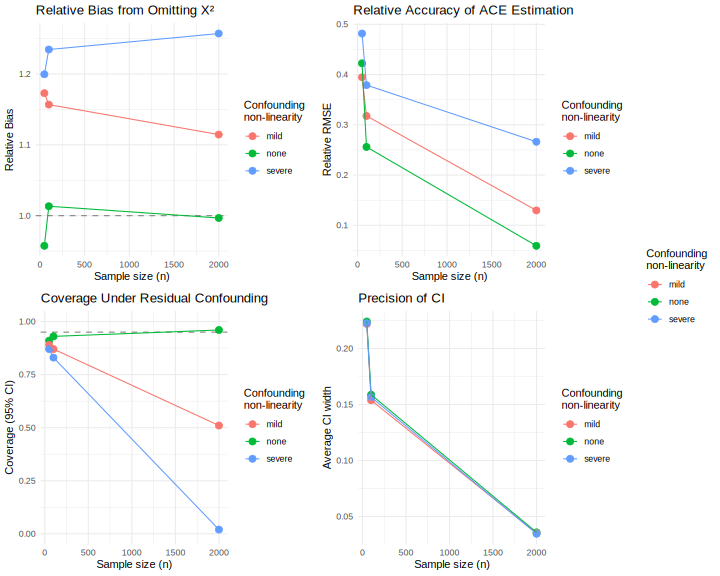
\includegraphics{article_files/figure-pdf/fig-performance-1.pdf}

}

\end{figure}%

\begin{table}

{\caption{{Performance metrics for ACE estimator across simulation
conditions}{\label{tbl-results}}}
\vspace{-20pt}}

\begin{longtable}[]{@{}
  >{\raggedright\arraybackslash}p{(\columnwidth - 10\tabcolsep) * \real{0.1600}}
  >{\centering\arraybackslash}p{(\columnwidth - 10\tabcolsep) * \real{0.1733}}
  >{\centering\arraybackslash}p{(\columnwidth - 10\tabcolsep) * \real{0.2000}}
  >{\centering\arraybackslash}p{(\columnwidth - 10\tabcolsep) * \real{0.2000}}
  >{\centering\arraybackslash}p{(\columnwidth - 10\tabcolsep) * \real{0.1333}}
  >{\centering\arraybackslash}p{(\columnwidth - 10\tabcolsep) * \real{0.1333}}@{}}
\toprule\noalign{}
\begin{minipage}[b]{\linewidth}\raggedright
Sample Size
\end{minipage} & \begin{minipage}[b]{\linewidth}\centering
Confounding
\end{minipage} & \begin{minipage}[b]{\linewidth}\centering
Relative Bias
\end{minipage} & \begin{minipage}[b]{\linewidth}\centering
Relative RMSE
\end{minipage} & \begin{minipage}[b]{\linewidth}\centering
Coverage
\end{minipage} & \begin{minipage}[b]{\linewidth}\centering
CI Width
\end{minipage} \\
\midrule\noalign{}
\endhead
\bottomrule\noalign{}
\endlastfoot
50 & none & 0.957 & 0.422 & 0.910 & 0.224 \\
100 & none & 1.013 & 0.256 & 0.930 & 0.159 \\
2000 & none & 0.997 & 0.059 & 0.960 & 0.036 \\
50 & mild & 1.173 & 0.395 & 0.890 & 0.222 \\
100 & mild & 1.157 & 0.318 & 0.870 & 0.154 \\
2000 & mild & 1.114 & 0.130 & 0.510 & 0.035 \\
50 & severe & 1.200 & 0.482 & 0.870 & 0.223 \\
100 & severe & 1.235 & 0.379 & 0.830 & 0.157 \\
2000 & severe & 1.257 & 0.266 & 0.020 & 0.035 \\
\end{longtable}

\end{table}

\subsubsection{Reproducing the Simulation and
Results}\label{reproducing-the-simulation-and-results}

As previously mentioned, researchers may not want or know how to use
dynamic document generation/literate programming. In this case, one
could still follow the same steps shown thus far focusing only on the .R
files while still benefiting from a reproducible computational
environment.

To illustrate it, after following Steps I-III, without needing to define
packages for the document rendering in Step I, the simulation study may
be reproduced (Listing~\ref{lst-run-simulation}) as follows:

\begin{codelisting}

\caption{\label{lst-run-simulation}Running the complete simulation
workflow \normalsize}

\centering{

\small

\begin{Shaded}
\begin{Highlighting}[]
\ExtensionTok{[nix{-}shell:\textasciitilde{}/Desktop/AMPPS/Why{-}risk{-}it{-}when{-}you{-}can{-}rix{-}it]$} 
  \ExtensionTok{Rscript}\NormalTok{ Simulation\_Scripts/03\_run\_simulation.R}
\end{Highlighting}
\end{Shaded}

}

\end{codelisting}%

In this same way one may also execute the .R file associated with the
performance criteria calculation and visualization. Therefore, the key
advantage of executing within \texttt{nix-shell} is that all
dependencies---R version, packages, and system tools---match exactly
those specified in \texttt{default.nix}.

\subsection{Additional Considerations for Advanced
Workflows}\label{additional-considerations-for-advanced-workflows}

\subsubsection{Workflow Orchestration: \{targets\} and
\{rixpress\}}\label{workflow-orchestration-targets-and-rixpress}

Complex simulation studies often benefit from workflow management
systems that track dependencies between computational steps, cache
intermediate results, and enable selective re-execution when inputs
change. Two complementary approaches exist within the Nix ecosystem:
using \{targets\} inside a Nix environment, or using \{rixpress\} to
leverage Nix itself as the build automation tool.

\paragraph{Using \{targets\} Within
Nix.}\label{using-targets-within-nix}

As mentioned, the \{targets\} package
(\citeproc{ref-landau_2021}{Landau, 2021}) provides workflow
orchestration for R-based projects. This combination ensures both
computational reproducibility (via Nix controlling the environment) and
computational efficiency (via targets' intelligent caching). To
integrate \{targets\} with Nix, simply include ``targets'' in the
\texttt{r\_pkgs} parameter of \texttt{rix()}, and execute the pipeline
within \texttt{nix-shell} using
\texttt{Rscript\ -e\ \textquotesingle{}targets::tar\_make()\textquotesingle{}}.
The \{targets\} metadata directory (\texttt{\_targets/}) should be
excluded from version control while the \texttt{\_targets.R}
configuration file should be committed alongside \texttt{default.nix}
(\citeproc{ref-rodrigues_baumann_2025}{Rodrigues \& Baumann, 2025}).
This approach is ideal for projects that remain within the R ecosystem
and do not require different computational environments for different
pipeline steps (see \{rix\} documentation:
\url{https://docs.ropensci.org/rix/articles/z-advanced-topic-reproducible-analytical-pipelines-with-nix.html}).

\paragraph{Using \{rixpress\} for Polyglot
Pipelines.}\label{using-rixpress-for-polyglot-pipelines}

The \{rixpress\} package (\citeproc{ref-rixpress}{Rodrigues, 2025}), a
sister package to \{rix\}, uses Nix itself as the build automation tool
rather than operating within a Nix environment. Each pipeline step
becomes a Nix derivation, providing hermetic builds with sandboxed
execution and content-addressable caching. The key advantage of
\{rixpress\} emerges in multi-language workflows: different steps can
execute in different Nix-defined environments (e.g., one step using R
4.2.0 with specific packages, another using Python 3.12 with machine
learning libraries, another using Julia for numerical optimization). The
package interface, inspired by \{targets\}, uses functions like
\texttt{rxp\_r()}, \texttt{rxp\_py()}, and \texttt{rxp\_jl()} to define
pipeline steps, with automatic serialization handling data transfer
between languages. Objects are stored in the Nix store and can be
inspected interactively using helper functions like \texttt{rxp\_read()}
and \texttt{rxp\_load()} (see \{rixpress\} documentation:
\url{https://docs.ropensci.org/rixpress/articles/intro-concepts.html}).

For the interested reader, in the GitHub repository we included a folder
in which the entire simulation and manuscript are produced using
\{rixpress\}.

\subsection{Converting Existing \{renv\}
Projects}\label{converting-existing-renv-projects}

Many researchers have existing projects using \{renv\} for package
management. The \texttt{renv2nix()} function facilitates migration by
reading an \texttt{renv.lock} file and generating an equivalent Nix
specification. This conversion is particularly valuable for projects
where \{renv\} encountered system dependency issues or where stricter
reproducibility guarantees are desired. However, researchers should note
that while \{renv\} snapshots R package versions, Nix additionally pins
system libraries and compilers, potentially exposing previously hidden
dependencies on system configuration
(\citeproc{ref-rodrigues_baumann_2025}{Rodrigues \& Baumann, 2025}) (see
\{rix\} documentation:
\url{https://docs.ropensci.org/rix/articles/f-renv2nix.html}).

\subsection{Containerization with
Docker}\label{containerization-with-docker}

Institutions with existing Docker-based infrastructure may wish to
combine Nix with containers. While this might seem redundant---both
technologies provide isolation---the combination offers complementary
benefits: Nix ensures bit-reproducible builds across systems, while
Docker provides a familiar deployment mechanism for non-Nix-aware
computing environments. The approach is to use Nix as the base layer
within a Docker container
(\citeproc{ref-rodrigues_baumann_2025}{Rodrigues \& Baumann, 2025}).
This strategy is particularly relevant, for example, for projects
requiring deployment to cloud computing platforms or high-performance
computing clusters where Docker is the standard containerization
technology (see \{rix\} documentation:
\url{https://docs.ropensci.org/rix/articles/z-advanced-topic-using-nix-inside-docker.html}).

\section{Discussion}\label{discussion}

Reproducibility in computational research is often treated as a matter
of transparency---making data and code available. This tutorial has
argued that transparency alone is insufficient without the ability to
reliably reconstruct the computational environments in which analyses
are executed. For simulation studies in particular, where results depend
critically on software versions, system libraries, and random number
generation, environment-level reproducibility is not optional but
essential.

By introducing Nix and the \{rix\} package, we demonstrated a practical
and accessible approach to fully specifying and rebuilding computational
environments for simulation-based research. This approach enables
analyses and manuscripts to be rerun identically across machines and
over time, transforming reproducibility from an aspirational goal into a
verifiable property of the research workflow.

Importantly, adopting environment reproducibility does not require
abandoning existing analytic practices. Nix is agnostic to programming
language, editor, workflow structure, and manuscript template, allowing
researchers to retain familiar tools while strengthening the reliability
of their work. In this sense, reproducible environments serve as
enabling infrastructure---supporting, rather than replacing, other best
practices such as version control, workflow orchestration, and
transparent reporting.

If reproducibility is to function as a cornerstone of cumulative
science, then the ability to reconstruct computational environments must
become a routine part of methodological practice. Tools such as Nix and
\{rix\} lower the barrier to achieving this goal, making fully
reproducible simulation research feasible without requiring deep systems
expertise. We hope this tutorial helps normalize environment-level
reproducibility as a standard component of rigorous computational
research in psychology and beyond.

\newpage{}

\section{References}\label{references}

\phantomsection\label{refs}
\begin{CSLReferences}{1}{0}
\bibitem[\citeproctext]{ref-baker_etall_2024}
Baker, D. H., Berg, M., Hansford, K., Quinn, B., Segala, F., \&
Warden-English, E. (2024). {ReproduceMe}: Lessons from a pilot project
on computational reproducibility. \emph{Meta-Psychology}, \emph{8},
MP.2023.4021. \url{https://doi.org/10.15626/MP.2023.4021}

\bibitem[\citeproctext]{ref-boettiger_2015}
Boettiger, C. (2015). An introduction to {Docker} for reproducible
research. \emph{ACM SIGOPS Operating Systems Review}, \emph{49}(1),
71--79. \url{https://doi.org/10.1145/2723872.2723882}

\bibitem[\citeproctext]{ref-boettiger_eddelbuettel_2017}
Boettiger, C., \& Eddelbuettel, D. (2017). An introduction to {Rocker}:
{Docker} containers for {R}. \emph{The R Journal}, \emph{9}(2),
527--536. \url{https://doi.org/10.32614/RJ-2017-065}

\bibitem[\citeproctext]{ref-dolstra_etall_2004}
Dolstra, E., De Jonge, M., \& Visser, E. (2004). Nix: A safe and
policy-free system for software deployment. \emph{18th Large
Installation System Administration Conference}, 79--92.

\bibitem[\citeproctext]{ref-feldman_1979}
Feldman, S. I. (1979). {Make} --- a program for maintaining computer
programs. \emph{Software: Practice and Experience}, \emph{9}(4),
255--265. \url{https://doi.org/10.1002/spe.4380090402}

\bibitem[\citeproctext]{ref-glatard_etall_2015}
Glatard, T., Lewis, L. B., Ferreira da Silva, R., Adalat, R., Beck, N.,
Lepage, C., Rioux, P., Rousseau, M.-É., Sherif, T., Deelman, E.,
Khalili-Mahani, N., \& Evans, A. C. (2015). Reproducibility of
neuroimaging analyses across operating systems. \emph{Frontiers in
Neuroinformatics}, \emph{9}, 12.
\url{https://doi.org/10.3389/fninf.2015.00012}

\bibitem[\citeproctext]{ref-hardwicke2020}
Hardwicke, T. E., Wallach, J. D., Kidwell, M. C., Bendixen, T., Crüwell,
S., \& Ioannidis, J. P. A. (2020). An empirical assessment of
transparency and reproducibility-related research practices in the
social sciences (2014{\textendash}2017). \emph{Royal Society Open
Science}, \emph{7}(2), 190806. \url{https://doi.org/10.1098/rsos.190806}

\bibitem[\citeproctext]{ref-hodges_etall_2023}
Hodges, C. B., Stone, B. M., Johnson, P. K., Carter, J. H., III,
Sawyers, C. K., Roby, P. R., \& Lindsey, H. M. (2023). Researcher
degrees of freedom in statistical software contribute to unreliable
results: A comparison of nonparametric analyses conducted in {SPSS},
{SAS}, {Stata}, and {R}. \emph{Behavior Research Methods}, \emph{55}(6),
2813--2837. \url{https://doi.org/10.3758/s13428-022-01932-2}

\bibitem[\citeproctext]{ref-kidwell_etall_2016}
Kidwell, M. C., Lazarević, L. B., Baranski, E., Hardwicke, T. E.,
Piechowski, S., Falkenberg, L.-S., Kennett, C., Slowik, A., Sonnleitner,
C., Hess-Holden, C., Errington, T. M., Fiedler, S., \& Nosek, B. A.
(2016). Badges to acknowledge open practices: A simple, low-cost,
effective method for increasing transparency. \emph{PLOS Biology},
\emph{14}(5), e1002456.
\url{https://doi.org/10.1371/journal.pbio.1002456}

\bibitem[\citeproctext]{ref-landau_2021}
Landau, W. M. (2021). \emph{Targets: Dynamic function-oriented make-like
declarative workflows}.

\bibitem[\citeproctext]{ref-levenstein_lyle_2018}
Levenstein, M. C., \& Lyle, J. A. (2018). Data: Sharing is caring.
\emph{Advances in Methods and Practices in Psychological Science},
\emph{1}(1), 95--103.

\bibitem[\citeproctext]{ref-luijken_etall_2024}
Luijken, K., Lohmann, A., Alter, U., Claramunt Gonzalez, J., Clouth, F.
J., Fossum, J. L., Hesen, L., Huizing, A. H. J., Ketelaar, J., Montoya,
A. K., Nab, L., Nijman, R. C. C., Penning de Vries, B. B. L., Tibbe, T.
D., Wang, Y. A., \& Groenwold, R. H. H. (2024). Replicability of
simulation studies for the investigation of statistical methods: The
{RepliSims} project. \emph{Royal Society Open Science}, \emph{11}(1),
231003. \url{https://doi.org/10.1098/rsos.231003}

\bibitem[\citeproctext]{ref-malka2024}
Malka, J., Zacchiroli, S., \& Zimmermann, T. (2024). Reproducibility of
build environments through space and time. \emph{Proceedings of the 2024
ACM/IEEE 44th International Conference on Software Engineering: New
Ideas and Emerging Results}, 97--101.
\url{https://doi.org/10.1145/3639476.3639767}

\bibitem[\citeproctext]{ref-morris_etall_2019}
Morris, T. P., White, I. R., \& Crowther, M. J. (2019). Using simulation
studies to evaluate statistical methods. \emph{Statistics in Medicine},
\emph{38}(11), 2074--2102. \url{https://doi.org/10.1002/sim.8086}

\bibitem[\citeproctext]{ref-rvinecopulib}
Nagler, T., \& Vatter, T. (2025). \emph{Rvinecopulib: High performance
algorithms for vine copula modeling}.
\url{https://CRAN.R-project.org/package=rvinecopulib}

\bibitem[\citeproctext]{ref-nosek_etall_2022}
Nosek, B. A., Hardwicke, T. E., Moshontz, H., Allard, A., Corker, K. S.,
Dreber, A., Fidler, F., Hilgard, J., Kline Struhl, M., Nuijten, M. B.,
Rohrer, J. M., Romero, F., Scheel, A. M., Scherer, L. D., Schönbrodt, F.
D., \& Vazire, S. (2022). Replicability, robustness, and reproducibility
in psychological science. \emph{Annual Review of Psychology}, \emph{73},
719--748. \url{https://doi.org/10.1146/annurev-psych-020821-114157}

\bibitem[\citeproctext]{ref-ottoboni_stark_2018}
Ottoboni, K., \& Stark, P. B. (2018). \emph{Random problems with r}.
\url{https://arxiv.org/abs/1809.06520}

\bibitem[\citeproctext]{ref-pawel_etall_2025}
Pawel, S., Bartoš, F., Siepe, B. S., \& Lohmann, A. (2025). Handling
missingness, failures, and non-convergence in simulation studies: A
review of current practices and recommendations. \emph{The American
Statistician}, 1--18.
\url{https://doi.org/10.1080/00031305.2025.2540002}

\bibitem[\citeproctext]{ref-peng_2011}
Peng, R. D. (2011). Reproducible research in computational science.
\emph{Science}, \emph{334}(6060), 1226--1227.

\bibitem[\citeproctext]{ref-rodrigues_2023}
Rodrigues, B. (2023). \emph{Building reproducible analytical pipelines
with {R}}. \url{https://raps-with-r.dev}

\bibitem[\citeproctext]{ref-rixpress}
Rodrigues, B. (2025). \emph{Rixpress: Build reproducible analytical
pipelines with 'nix'}. \url{https://CRAN.R-project.org/package=rixpress}

\bibitem[\citeproctext]{ref-rodrigues_baumann_2025}
Rodrigues, B., \& Baumann, P. (2025). \emph{Rix: Reproducible data
science environments with 'nix'}.
\url{https://CRAN.R-project.org/package=rix}

\bibitem[\citeproctext]{ref-rodrigues_baumann_2026_polyglot}
Rodrigues, B., \& Baumann, P. (2026). \emph{Nix for polyglot,
reproducible data science workflows} (Version v0.0.1). Zenodo.
\url{https://doi.org/10.5281/zenodo.18138618}

\bibitem[\citeproctext]{ref-schneider_2024}
Schneider, W. J. (2024). \emph{{Apaquarto}} {[}Computer software{]}.
\url{https://github.com/wjschne/apaquarto}

\bibitem[\citeproctext]{ref-siepe_etall_2024}
Siepe, B. S., Bartoš, F., Morris, T. P., Boulesteix, A.-L., Heck, D. W.,
\& Pawel, S. (2024). Simulation studies for methodological research in
psychology: A standardized template for planning, preregistration, and
reporting. \emph{Psychological Methods}.
\url{https://doi.org/10.1037/met0000695}

\bibitem[\citeproctext]{ref-simonsohn_2020}
Simonsohn, U. (2020). \emph{Groundhog: Version-control for CRAN, github,
and gitlab packages}.

\bibitem[\citeproctext]{ref-ushey_2024}
Ushey, K. (2024). \emph{Renv: Project environments}.

\bibitem[\citeproctext]{ref-vazire2018}
Vazire, S. (2018). Implications of the Credibility Revolution for
Productivity, Creativity, and Progress. \emph{Perspectives on
Psychological Science}, \emph{13}(4), 411--417.
\url{https://doi.org/10.1177/1745691617751884}

\bibitem[\citeproctext]{ref-white_etall_2024}
White, I. R., Pham, T. M., Quartagno, M., \& Morris, T. P. (2024). How
to check a simulation study. \emph{International Journal of
Epidemiology}, \emph{53}(1), dyad134.
\url{https://doi.org/10.1093/ije/dyad134}

\end{CSLReferences}

\appendix

\section{Simulation Study Design}\label{apx-simulation-study-design}

Here we present a rather short description following recommendations
from previous research, but ideally even more may be reported
(\citeproc{ref-morris_etall_2019}{Morris et al., 2019};
\citeproc{ref-pawel_etall_2025}{Pawel et al., 2025};
\citeproc{ref-siepe_etall_2024}{Siepe et al., 2024};
\citeproc{ref-white_etall_2024}{White et al., 2024}). This mimics a
methods or similar section in articles.

\textbf{Factorial Design.} The simulation employs a full factorial
design with two factors: sample size (\(n \in \{50, 100, 2000\}\)) and
degree of confounding non-linearity (\(\gamma_2 \in \{0, 0.3, 0.8\}\),
labeled as none, mild, and severe). The parameter \(\gamma_2\) controls
the strength of the quadratic confounder effect on the outcome (see Data
Generation). This yields nine conditions, each replicated \(K = 1000\)
times.

\textbf{Data Generation.} For each replication, data are generated
following a causal structure where a confounder \(X_2\) affects both
treatment assignment and the outcome. The confounder and treatment error
term are generated using the \{rvinecopulib\} package: pairs
\((U_1, U_2)\) are drawn from an independence copula via
\texttt{rbicop()}, then transformed to standard normals via
\(X_2 = \Phi^{-1}(U_1)\) and \(\epsilon = \Phi^{-1}(U_2)\). The
independence copula is simply \(C(u,v) = uv\), meaning the resulting
uniforms are independent---mathematically equivalent to calling
\texttt{rnorm()} directly. We use \{rvinecopulib\} intentionally because
it depends on C++ libraries.

Treatment assignment follows
\(X_1 = \alpha_0 + \alpha_1 X_2 + \alpha_2 X_2^2 + \epsilon\) where
\(\alpha_0 = 0\), \(\alpha_1 = 0.5\), and \(\alpha_2 = 0.2\). This
creates confounding because \(X_2\) influences treatment assignment
through both linear and quadratic terms. The binary outcome is generated
from the true logistic regression model: \[
\text{logit}(P(Y = 1 \mid X_1, X_2)) = \beta_0 + \beta_1 X_1 + \gamma_1 X_2 + \gamma_2 X_2^2
\]

\noindent with parameters \(\beta_0 = -0.5\), \(\beta_1 = 0.7\) (the
causal effect of interest), \(\gamma_1 = -0.4\), and \(\gamma_2\)
varying by condition. The analyst misspecifies the outcome model by
omitting the quadratic confounder term, fitting instead: \[
\text{logit}(P(Y = 1 \mid X_1, X_2)) = \beta_0 + \beta_1 X_1 + \gamma_1 X_2
\]

This misspecification creates residual confounding because the omitted
term \(\gamma_2 X_2^2\) is correlated with \(X_1\) (since \(X_1\)
depends on both \(X_2\) and \(X_2^2\)), violating the conditional
exchangeability assumption given linear adjustment alone.

\textbf{Estimand.} The target estimand is the average causal effect
(ACE) of \(X_1\) on \(Y\), properly adjusted for confounding: \[
\text{ACE}(X_1) = \mathbb{E}\left[\frac{\partial P(Y = 1 \mid X_1, X_2)}{\partial X_1}\right] = \mathbb{E}\left[\beta_1 \cdot \frac{\exp(\eta)}{(1 + \exp(\eta))^2}\right]
\]

\noindent where
\(\eta = \beta_0 + \beta_1 X_1 + \gamma_1 X_2 + \gamma_2 X_2^2\) is the
correctly specified linear predictor, and the expectation is taken over
the joint distribution of \((X_1, X_2)\). For each \(\gamma_2\)
condition, the ``true'' ACE (denoted \(\theta\)) is approximated once
using a very large sample (\(N = 200,000\)) with the correctly specified
model including \(X_2^2\).

\textbf{Estimator.} The causal effect is estimated from the misspecified
model (omitting \(X_2^2\)) as: \[
\widehat{\text{ACE}}(X_1) = \frac{1}{n}\sum_{i=1}^{n} \tilde{\beta}_1 \cdot \frac{\exp(\tilde{\eta}_i)}{(1 + \exp(\tilde{\eta}_i))^2}
\]

\noindent where
\(\tilde{\eta}_i = \tilde{\beta}_0 + \tilde{\beta}_1 X_{i1} + \tilde{\gamma}_1 X_{i2}\)
and
\(\tilde{\boldsymbol{\beta}} = (\tilde{\beta}_0, \tilde{\beta}_1, \tilde{\gamma}_1)\)
are maximum likelihood estimates from the misspecified logistic
regression.

\begin{longtable}[]{@{}
  >{\raggedright\arraybackslash}p{(\columnwidth - 4\tabcolsep) * \real{0.3333}}
  >{\raggedright\arraybackslash}p{(\columnwidth - 4\tabcolsep) * \real{0.3333}}
  >{\raggedright\arraybackslash}p{(\columnwidth - 4\tabcolsep) * \real{0.3333}}@{}}
\caption{Performance criteria for evaluating the ACE estimator.
\(\hat{\theta}_k\) denotes the ACE estimate from replication \(k\) (for
\(k = 1, \ldots, K\)), where \(K = 1000\) is the number of replications,
and \(\theta\) denotes the true ACE for a given condition. For coverage
and width criteria, \(A_k\) and \(B_k\) denote the lower and upper
endpoints of the 95\% confidence interval from replication \(k\),
\(W_k = B_k - A_k\) is the interval width, \(c_{\beta}\) is the
estimated coverage probability, and \(I(\cdot)\) is an indicator
function equaling 1 if the condition is true and 0 otherwise. The Monte
Carlo standard error (MCSE) quantifies the simulation uncertainty in
each performance measure estimate}\tabularnewline
\toprule\noalign{}
\begin{minipage}[b]{\linewidth}\raggedright
Criterion
\end{minipage} & \begin{minipage}[b]{\linewidth}\raggedright
Estimate
\end{minipage} & \begin{minipage}[b]{\linewidth}\raggedright
MCSE
\end{minipage} \\
\midrule\noalign{}
\endfirsthead
\toprule\noalign{}
\begin{minipage}[b]{\linewidth}\raggedright
Criterion
\end{minipage} & \begin{minipage}[b]{\linewidth}\raggedright
Estimate
\end{minipage} & \begin{minipage}[b]{\linewidth}\raggedright
MCSE
\end{minipage} \\
\midrule\noalign{}
\endhead
\bottomrule\noalign{}
\endlastfoot
Bias & \(\frac{1}{K}\sum_{k=1}^K \hat{\theta}_k - \theta\) &
\(\sqrt{\frac{1}{K(K-1)}\sum_{k=1}^K(\hat{\theta}_k - \bar{\hat{\theta}})^2}\) \\
Variance &
\(\frac{1}{K-1}\sum_{k=1}^K(\hat{\theta}_k - \bar{\hat{\theta}})^2\) &
\(\sqrt{\frac{K-1}{K}}\cdot\frac{1}{K-1}\sum_{k=1}^K(\hat{\theta}_k - \bar{\hat{\theta}})^2\) \\
RMSE & \(\sqrt{\frac{1}{K}\sum_{k=1}^K (\hat{\theta}_k - \theta)^2}\) &
\(\sqrt{\frac{K-1}{K}\sum_{j=1}^K\left(\sqrt{(\hat{\theta}_j - \theta)^2} - \overline{RMSE}\right)^2}\) \\
Relative Bias & \(\frac{1}{\theta K}\sum_{k=1}^K \hat{\theta}_k\) &
\(\frac{1}{\theta}\sqrt{\frac{1}{K(K-1)}\sum_{k=1}^K(\hat{\theta}_k - \bar{\hat{\theta}})^2}\) \\
Relative RMSE &
\(\frac{1}{\theta}\sqrt{\frac{1}{K}\sum_{k=1}^K (\hat{\theta}_k - \theta)^2}\)
&
\(\frac{1}{\theta}\sqrt{\frac{K-1}{K}\sum_{j=1}^K\left(\sqrt{(\hat{\theta}_j - \theta)^2} - \overline{RMSE}\right)^2}\) \\
Coverage & \(\frac{1}{K}\sum_{k=1}^K I(A_k \leq \theta \leq B_k)\) &
\(\sqrt{\frac{c_{\beta}(1 - c_{\beta})}{K}}\) \\
Width & \(\frac{1}{K}\sum_{k=1}^K (B_k - A_k)\) &
\(\sqrt{\frac{1}{K(K-1)}\sum_{k=1}^K(W_k - \bar{W})^2}\) \\
\end{longtable}

\textbf{Performance Criteria.} Table 1 presents the performance criteria
used to evaluate the ACE estimator across simulation conditions.

\textbf{Computational Details.} The simulation was conducted on a
MacBook Pro (\ldots), running macOS Sequoia 15.6.1. All analyses were
performed in R (version 4.4.3). Parallel processing was implemented
through the \{doParallel\} package (version 1.0.17), with \{doRNG\}
(version 1.8.6.2) to ensure independent and reproducible random number
streams. For data generation we used the \{rvinecopulib\} package
(version 0.7.3.1.0). The estimator was implemented using the
\{marginaleffects\} package (version 0.31.0). Data wrangling was
performed with \{dplyr\} (version 1.1.4). Method performance was
assessed through multiple metrics following the formulas from the
\{simhelpers\} package (version 0.3.1). Figures were produced with
\{ggplot2\} (version 4.0.1) and \{cowplot\} (version 1.1.3).

\section{Clarifying the packages
used}\label{apx-clarifying-the-packages-used}






\end{document}
